% Options for packages loaded elsewhere
\PassOptionsToPackage{unicode}{hyperref}
\PassOptionsToPackage{hyphens}{url}
\PassOptionsToPackage{dvipsnames,svgnames*,x11names*}{xcolor}
%
\documentclass[
  12pt,
]{article}
\usepackage{lmodern}
\usepackage{amssymb,amsmath}
\usepackage{ifxetex,ifluatex}
\ifnum 0\ifxetex 1\fi\ifluatex 1\fi=0 % if pdftex
  \usepackage[T1]{fontenc}
  \usepackage[utf8]{inputenc}
  \usepackage{textcomp} % provide euro and other symbols
\else % if luatex or xetex
  \usepackage{unicode-math}
  \defaultfontfeatures{Scale=MatchLowercase}
  \defaultfontfeatures[\rmfamily]{Ligatures=TeX,Scale=1}
\fi
% Use upquote if available, for straight quotes in verbatim environments
\IfFileExists{upquote.sty}{\usepackage{upquote}}{}
\IfFileExists{microtype.sty}{% use microtype if available
  \usepackage[]{microtype}
  \UseMicrotypeSet[protrusion]{basicmath} % disable protrusion for tt fonts
}{}
\makeatletter
\@ifundefined{KOMAClassName}{% if non-KOMA class
  \IfFileExists{parskip.sty}{%
    \usepackage{parskip}
  }{% else
    \setlength{\parindent}{0pt}
    \setlength{\parskip}{6pt plus 2pt minus 1pt}}
}{% if KOMA class
  \KOMAoptions{parskip=half}}
\makeatother
\usepackage{xcolor}
\IfFileExists{xurl.sty}{\usepackage{xurl}}{} % add URL line breaks if available
\IfFileExists{bookmark.sty}{\usepackage{bookmark}}{\usepackage{hyperref}}
\hypersetup{
  pdftitle={Assignment FSE},
  pdfauthor={Dorian Quelle \& Frederic Denker},
  colorlinks=true,
  linkcolor=Maroon,
  filecolor=Maroon,
  citecolor=Blue,
  urlcolor=blue,
  pdfcreator={LaTeX via pandoc}}
\urlstyle{same} % disable monospaced font for URLs
\usepackage[margin=3cm]{geometry}
\usepackage{graphicx,grffile}
\makeatletter
\def\maxwidth{\ifdim\Gin@nat@width>\linewidth\linewidth\else\Gin@nat@width\fi}
\def\maxheight{\ifdim\Gin@nat@height>\textheight\textheight\else\Gin@nat@height\fi}
\makeatother
% Scale images if necessary, so that they will not overflow the page
% margins by default, and it is still possible to overwrite the defaults
% using explicit options in \includegraphics[width, height, ...]{}
\setkeys{Gin}{width=\maxwidth,height=\maxheight,keepaspectratio}
% Set default figure placement to htbp
\makeatletter
\def\fps@figure{htbp}
\makeatother
\setlength{\emergencystretch}{3em} % prevent overfull lines
\providecommand{\tightlist}{%
  \setlength{\itemsep}{0pt}\setlength{\parskip}{0pt}}
\setcounter{secnumdepth}{-\maxdimen} % remove section numbering
\usepackage{dcolumn}
\usepackage{setspace}
\doublespacing
\usepackage[utf8]{inputenc}
\usepackage{float}
\usepackage{xcolor}
\usepackage{lipsum}

\title{Assignment FSE}
\author{Dorian Quelle \& Frederic Denker}
\date{Juli 19, 2020}

\begin{document}
\maketitle

\hypertarget{research-summary}{%
\subsection{Research Summary:}\label{research-summary}}

\hypertarget{keywords}{%
\subsection{Keywords}\label{keywords}}

Factorial survey experiment, donation, nudging

\newpage

\hypertarget{introduction}{%
\subsection{Introduction}\label{introduction}}

What, why and how?

\hypertarget{theory}{%
\subsection{Theory:}\label{theory}}

Relevant Theories, Hypnosis building

\hypertarget{method}{%
\subsection{Method}\label{method}}

Why FSE?

The next part will give short description of the survey methodology
itsself:

The initial planning was to run this experiment as Pen-and-Paper
Personal Interviews (PAPI). Due to the Covid-19 Pandemic this was not
feasible anymore. Therefore, we resorted to sending the PDF of the
questionnaires to the respondents and asking them to print it and send
it back.

When creating the questionnaires a sampling strategy needs to be
employed. However, our survey only has 5 dimensions with 3,3,3,2,2
levels. This means that we have a universe of 108 unique vignettes.
Including 12 vignettes for each survey we able to survey the complete
universe of vignettes in 9 surveys. We surveyed 17 individuals and each
deck at least once which should increases the validity.

\hypertarget{operationalization}{%
\subsection{Operationalization}\label{operationalization}}

For each of the twelve vignettes we presented the respondent with five
dimensions for which he or she had to respond to the question \emph{How
likely is it that you are going to donate the amount?} The following
dimensions were:

\begin{itemize}
\tightlist
\item
  The working situation of the person who will be asked to donate. The
  available options are a minimum wage job and a well paying job.
\item
  The amount of money you receive. It can be either 10, 100 or 1000
  Euros.
\item
  The origin of the money. The available options were tax refund, gift
  from mother or a bonus from work.
\item
  The channel of the money. This differentiates between whether you have
  yet to receive the money and can decide to redirect it to the cause or
  whether you have already received the money.
\item
  Lastly, the goal of the donation which can be building state capacity
  in Uganda, supporting small businesses and entrepreneurs in Uganda or
  provide education for young mothers in Uganda.
\end{itemize}

The respondent is then asked about their likelihood of donating using a
Likert Scale with 5 values. The extremes (-2 and 2) were labeled ``Very
unlikely'' and ``Very likely'' respectively.

Below you will find one example vignette as it was presented to the
respondents:

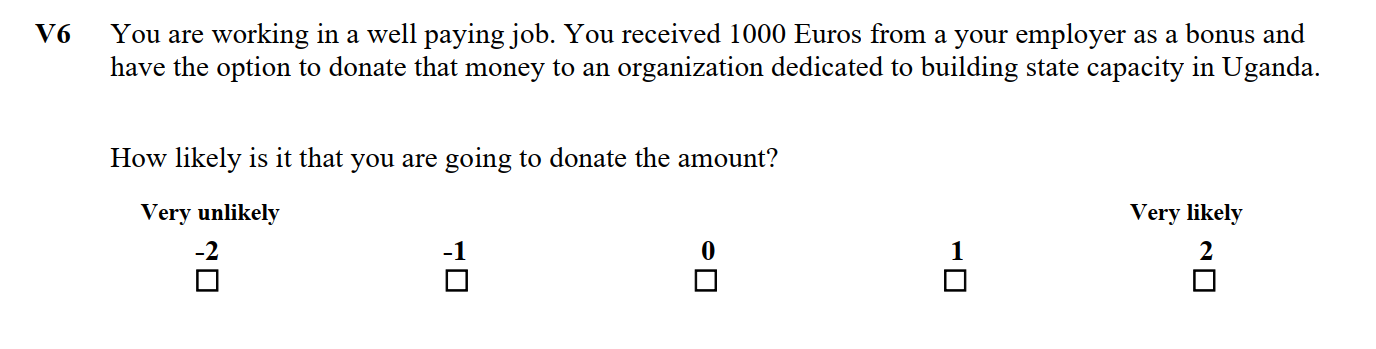
\includegraphics[width=1.05\linewidth]{Screenshot_vignette}

In addition to these 12 vignettes we asked the respondents to answer 5
questions on themselves, more specifically gender, year of birth,
country of residence and highest educational qualification.

\hypertarget{theoretical-background-and-relevance}{%
\subsection{Theoretical Background and
Relevance}\label{theoretical-background-and-relevance}}

\hypertarget{relevance}{%
\subsubsection{Relevance}\label{relevance}}

Donations for humanitarian purposes are essential for many organizations
and regions of the world. There is much research in the literature to
understand why and how people donate money. VGL XXX. Although there are
discussions about the efficiency and long-term effects of charitable
donations and foreign aid (SACHS ZITIEREN), millions of people, through
no fault of their own, find themselves in situations where donations are
essential for survival. From this fact and the mandate of the UN
Universal Declaration of Human Rights (ART 1 and 3) ``All human beings
are born free and equal in dignity and rights'', ``Everyone has the
right to life, liberty and security of person''. it follows that at this
point in time it is not possible to refrain from making donations. In
this study we will not talk about the moral and economic implications of
donations, but we will assume that they are necessary. We are only
interested in understanding why people donate and what they donate for.
The results of this experiment will help charitable organizations to
better adapt fundraising to their specific circumstances. This should
maximize the amount of money donated to charity.

\hypertarget{the-factorial-survey-methodology}{%
\subsubsection{The Factorial Survey
Methodology}\label{the-factorial-survey-methodology}}

Ample research is based on empirical analyses of the donation behavior
of specific population groups. XXX While this approach reflects reality
more accurately because it takes unobserved factors into account when
individuals make decisions, it is precisely here that the weakness of
this analysis technique lies. (XXX) Although Factorial Surveys are not a
new approach in the field, we believe that our approach deserves some
attention. Through a Factorial Survey it is possible to combine the
advantages of an experiment with those of a questionnaire. This means
that although the number of participants is significantly higher than in
a laboratory experiment, causal statements can be made by allowing the
researchers to control all factors.

\hypertarget{theoretical-background}{%
\subsubsection{Theoretical Background}\label{theoretical-background}}

In this section we will explain the theoretical connections of
individual variables and dimensions with the willingness to donate. The
first variable is the origin of the money that the participant should
imagine to have received. Several authors have already investigated how
different origins of money can change the probability and amount of a
donation. For example, Steinberg et al.~find in their study
``Inheritance and Charitable Donations'' that inherited money has a
significantly higher elasticity in donations than earned money. The
theoretical argumentation used by the authors is the ``Mental Accounting
Theory'' according to Shefrin and Thaler. Mental accounting is used in
behavioural economics as an approach to explain the varying handling of
different (objectively often equivalent) financial transactions.
Thaler's analyses for empirical anomalies in orthodox economics and his
analysis of mental accounting earned him a Nobel Prize in 2017.
Accordingly, his theories are widely accepted and represent the modern
basis for behavioural economics. In our study the variable takes the
values:

\begin{itemize}
\tightlist
\item
  Tax refund
\item
  Bonus
\item
  Gift from mother
\end{itemize}

The tax refund is a windfall gain where we expect the elasticity of the
donations to be relatively high. (XXX) Furthermore, the variable should
point out the positive aspects of a nation state (REVISION) and thus be
linked to the aim of the donation. The interaction with the objectives
of the donation will be examined in more detail at a later stage. The
second variable, the bonus, represents the origin ``earned money''.
Since the money itself was earned here, we assume that there will be a
significantly lower elasticity and willingness to donate. Because people
feel as if they have a claim to the money. Furthermore, studies have
already confirmed that people are driven into a ``market mode'' by
self-earned money. Here people become less cooperative and less social.
They live more according to the motto: ``When everyone thinks of
themselves, everyone is thought of.''(BBE LAST SESSION + REVISION)
Lastly, we will focus on the expression ``gift of the mother''. A gift
from the mother is a windfall gain but is often connected with the norm
that the money is spent for the own or common good. Therefore we expect
that the willingness to donate will decrease. (REVISING)

In summary, our hypotheses regarding the first variable are:

\begin{itemize}
\tightlist
\item
  H1a: \(\beta_{taxrefund} > 0\)
\item
  H1b: \(\beta_{earnedmodey} < 0\)
\item
  H1c: \(\beta_{giftfrommother} < 0\)
\end{itemize}

\hypertarget{results}{%
\subsection{Results}\label{results}}

Before looking at inferential statistics it is essential to get an
overview over the data, starting with the properties of the respondents
themsselves:

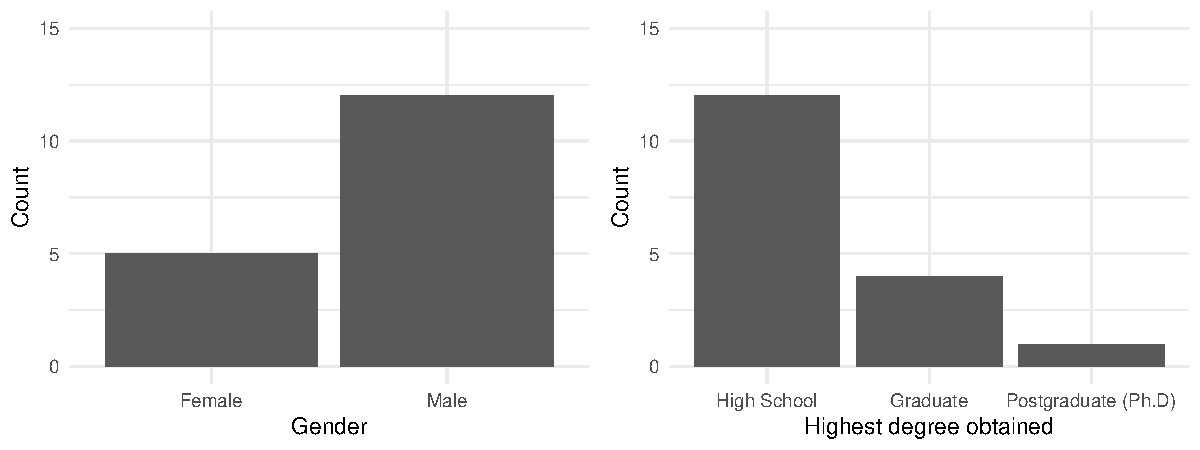
\includegraphics[width=1.05\linewidth]{FSE_paper_files/figure-latex/unnamed-chunk-2-1}

In order to give a short display of the data, the distribution of the
main outcome variable is plotted below:

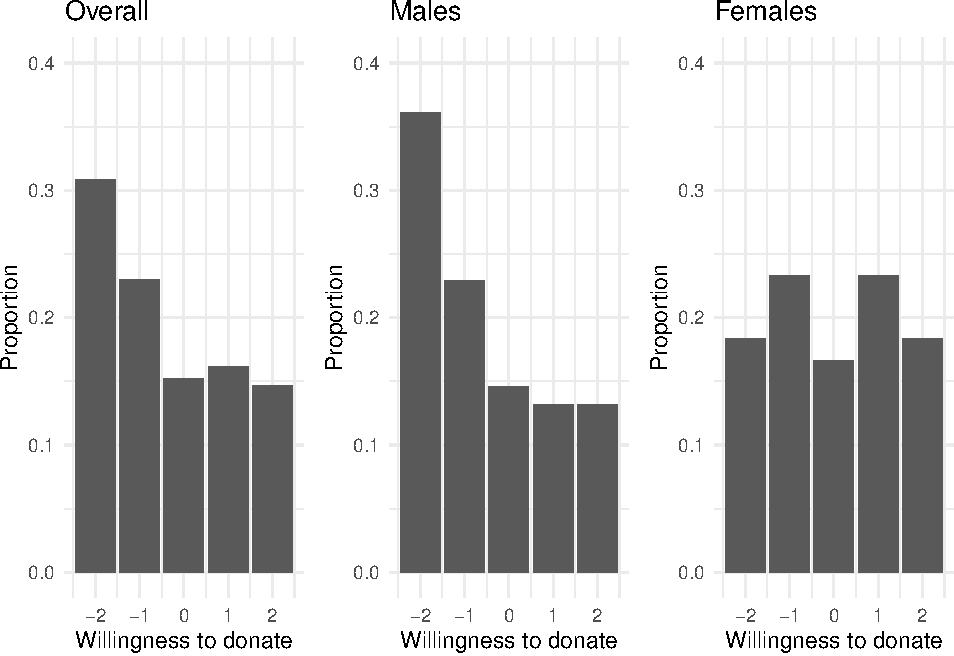
\includegraphics{FSE_paper_files/figure-latex/plotting_proportions-1.pdf}

\hypertarget{discussion}{%
\subsection{Discussion}\label{discussion}}

\end{document}
